\documentclass[12pt,letterpaper]{hmcpset}
\usepackage[margin=1in]{geometry}
\usepackage{graphicx}
\usepackage{amsthm}
\usepackage{enumitem}

% Theorems
\usepackage{amsthm}
\renewcommand\qedsymbol{$\blacksquare$}
\makeatletter
\@ifclassloaded{article}{
    \newtheorem{definition}{Definition}[section]
    \newtheorem{example}{Example}[section]
    \newtheorem{theorem}{Theorem}[section]
    \newtheorem{corollary}{Corollary}[theorem]
    \newtheorem{lemma}{Lemma}[theorem]
}{
}
\makeatother

% Random Stuff
\setlength\unitlength{1mm}

\newcommand{\insertfig}[3]{
\begin{figure}[htbp]\begin{center}\begin{picture}(120,90)
\put(0,-5){\includegraphics[width=12cm,height=9cm,clip=]{#1.eps}}\end{picture}\end{center}
\caption{#2}\label{#3}\end{figure}}

\newcommand{\insertxfig}[4]{
\begin{figure}[htbp]
\begin{center}
\leavevmode \centerline{\resizebox{#4\textwidth}{!}{\input
#1.pstex_t}}
\caption{#2} \label{#3}
\end{center}
\end{figure}}

\long\def\comment#1{}

\newcommand\norm[1]{\left\lVert#1\right\rVert}
\DeclareMathOperator*{\argmin}{arg\,min}
\DeclareMathOperator*{\argmax}{arg\,max}

% bb font symbols
\newfont{\bbb}{msbm10 scaled 700}
\newcommand{\CCC}{\mbox{\bbb C}}

\newfont{\bbf}{msbm10 scaled 1100}
\newcommand{\CC}{\mbox{\bbf C}}
\newcommand{\PP}{\mbox{\bbf P}}
\newcommand{\RR}{\mbox{\bbf R}}
\newcommand{\QQ}{\mbox{\bbf Q}}
\newcommand{\ZZ}{\mbox{\bbf Z}}
\renewcommand{\SS}{\mbox{\bbf S}}
\newcommand{\FF}{\mbox{\bbf F}}
\newcommand{\GG}{\mbox{\bbf G}}
\newcommand{\EE}{\mbox{\bbf E}}
\newcommand{\NN}{\mbox{\bbf N}}
\newcommand{\KK}{\mbox{\bbf K}}
\newcommand{\KL}{\mbox{\bbf KL}}

% Vectors
\renewcommand{\aa}{{\bf a}}
\newcommand{\bb}{{\bf b}}
\newcommand{\cc}{{\bf c}}
\newcommand{\dd}{{\bf d}}
\newcommand{\ee}{{\bf e}}
\newcommand{\ff}{{\bf f}}
\renewcommand{\gg}{{\bf g}}
\newcommand{\hh}{{\bf h}}
\newcommand{\ii}{{\bf i}}
\newcommand{\jj}{{\bf j}}
\newcommand{\kk}{{\bf k}}
\renewcommand{\ll}{{\bf l}}
\newcommand{\mm}{{\bf m}}
\newcommand{\nn}{{\bf n}}
\newcommand{\oo}{{\bf o}}
\newcommand{\pp}{{\bf p}}
\newcommand{\qq}{{\bf q}}
\newcommand{\rr}{{\bf r}}
\renewcommand{\ss}{{\bf s}}
\renewcommand{\tt}{{\bf t}}
\newcommand{\uu}{{\bf u}}
\newcommand{\ww}{{\bf w}}
\newcommand{\vv}{{\bf v}}
\newcommand{\xx}{{\bf x}}
\newcommand{\yy}{{\bf y}}
\newcommand{\zz}{{\bf z}}
\newcommand{\0}{{\bf 0}}
\newcommand{\1}{{\bf 1}}

% Matrices
\newcommand{\Ab}{{\bf A}}
\newcommand{\Bb}{{\bf B}}
\newcommand{\Cb}{{\bf C}}
\newcommand{\Db}{{\bf D}}
\newcommand{\Eb}{{\bf E}}
\newcommand{\Fb}{{\bf F}}
\newcommand{\Gb}{{\bf G}}
\newcommand{\Hb}{{\bf H}}
\newcommand{\Ib}{{\bf I}}
\newcommand{\Jb}{{\bf J}}
\newcommand{\Kb}{{\bf K}}
\newcommand{\Lb}{{\bf L}}
\newcommand{\Mb}{{\bf M}}
\newcommand{\Nb}{{\bf N}}
\newcommand{\Ob}{{\bf O}}
\newcommand{\Pb}{{\bf P}}
\newcommand{\Qb}{{\bf Q}}
\newcommand{\Rb}{{\bf R}}
\newcommand{\Sb}{{\bf S}}
\newcommand{\Tb}{{\bf T}}
\newcommand{\Ub}{{\bf U}}
\newcommand{\Wb}{{\bf W}}
\newcommand{\Vb}{{\bf V}}
\newcommand{\Xb}{{\bf X}}
\newcommand{\Yb}{{\bf Y}}
\newcommand{\Zb}{{\bf Z}}

% Calligraphic
\newcommand{\Ac}{{\cal A}}
\newcommand{\Bc}{{\cal B}}
\newcommand{\Cc}{{\cal C}}
\newcommand{\Dc}{{\cal D}}
\newcommand{\Ec}{{\cal E}}
\newcommand{\Fc}{{\cal F}}
\newcommand{\Gc}{{\cal G}}
\newcommand{\Hc}{{\cal H}}
\newcommand{\Ic}{{\cal I}}
\newcommand{\Jc}{{\cal J}}
\newcommand{\Kc}{{\cal K}}
\newcommand{\Lc}{{\cal L}}
\newcommand{\Mc}{{\cal M}}
\newcommand{\Nc}{{\cal N}}
\newcommand{\Oc}{{\cal O}}
\newcommand{\Pc}{{\cal P}}
\newcommand{\Qc}{{\cal Q}}
\newcommand{\Rc}{{\cal R}}
\newcommand{\Sc}{{\cal S}}
\newcommand{\Tc}{{\cal T}}
\newcommand{\Uc}{{\cal U}}
\newcommand{\Wc}{{\cal W}}
\newcommand{\Vc}{{\cal V}}
\newcommand{\Xc}{{\cal X}}
\newcommand{\Yc}{{\cal Y}}
\newcommand{\Zc}{{\cal Z}}

% Bold greek letters
\newcommand{\alphab}{\hbox{\boldmath$\alpha$}}
\newcommand{\betab}{\hbox{\boldmath$\beta$}}
\newcommand{\gammab}{\hbox{\boldmath$\gamma$}}
\newcommand{\deltab}{\hbox{\boldmath$\delta$}}
\newcommand{\etab}{\hbox{\boldmath$\eta$}}
\newcommand{\lambdab}{\hbox{\boldmath$\lambda$}}
\newcommand{\epsilonb}{\hbox{\boldmath$\epsilon$}}
\newcommand{\nub}{\hbox{\boldmath$\nu$}}
\newcommand{\mub}{\hbox{\boldmath$\mu$}}
\newcommand{\zetab}{\hbox{\boldmath$\zeta$}}
\newcommand{\phib}{\hbox{\boldmath$\phi$}}
\newcommand{\psib}{\hbox{\boldmath$\psi$}}
\newcommand{\thetab}{\hbox{\boldmath$\theta$}}
\newcommand{\taub}{\hbox{\boldmath$\tau$}}
\newcommand{\omegab}{\hbox{\boldmath$\omega$}}
\newcommand{\xib}{\hbox{\boldmath$\xi$}}
\newcommand{\sigmab}{\hbox{\boldmath$\sigma$}}
\newcommand{\pib}{\hbox{\boldmath$\pi$}}
\newcommand{\rhob}{\hbox{\boldmath$\rho$}}

\newcommand{\Gammab}{\hbox{\boldmath$\Gamma$}}
\newcommand{\Lambdab}{\hbox{\boldmath$\Lambda$}}
\newcommand{\Deltab}{\hbox{\boldmath$\Delta$}}
\newcommand{\Sigmab}{\hbox{\boldmath$\Sigma$}}
\newcommand{\Phib}{\hbox{\boldmath$\Phi$}}
\newcommand{\Pib}{\hbox{\boldmath$\Pi$}}
\newcommand{\Psib}{\hbox{\boldmath$\Psi$}}
\newcommand{\Thetab}{\hbox{\boldmath$\Theta$}}
\newcommand{\Omegab}{\hbox{\boldmath$\Omega$}}
\newcommand{\Xib}{\hbox{\boldmath$\Xi$}}

% mixed symbols
\newcommand{\sinc}{{\hbox{sinc}}}
\newcommand{\diag}{{\hbox{diag}}}
\renewcommand{\det}{{\hbox{det}}}
\newcommand{\trace}{{\hbox{tr}}}
\newcommand{\tr}{\trace}
\newcommand{\sign}{{\hbox{sign}}}
\renewcommand{\arg}{{\hbox{arg}}}
\newcommand{\var}{{\hbox{var}}}
\newcommand{\cov}{{\hbox{cov}}}
\renewcommand{\Re}{{\rm Re}}
\renewcommand{\Im}{{\rm Im}}
\newcommand{\eqdef}{\stackrel{\Delta}{=}}
\newcommand{\defines}{{\,\,\stackrel{\scriptscriptstyle \bigtriangleup}{=}\,\,}}
\newcommand{\<}{\left\langle}
\renewcommand{\>}{\right\rangle}
\newcommand{\Psf}{{\sf P}}
\newcommand{\T}{\top}
\newcommand{\m}[1]{\begin{bmatrix} #1 \end{bmatrix}}


% info for header block in upper right hand corner
\name{Eli Weissler}
\class{Math189R SP19}
\assignment{Homework 1}
\duedate{Monday, February 03, 2019}

\renewcommand{\labelenumi}{{(\alph{enumi})}}


\begin{document}
Feel free to work with other students, but make sure you write up the homework
and code on your own (no copying homework \textit{or} code; no pair programming).
Feel free to ask students or instructors for help debugging code or whatever else,
though.
The starter code for problem 2 part c and d can be found under the Resource tab on course website.\\

\textit{Note:} You need to create a Github account for submission of the coding part of the homework. Please create a repository on Github to hold all your code and include your Github account username as part of the answer to problem 2.

\begin{problem}[1]
(\textbf{Linear Transformation}) Let $\mathbf{y} = A\mathbf{x} + \mathbf{b}$ be a random vector.
show that expectation is linear:
\[
    \EE[\yy] = \EE[A\xx + \bb] = A\EE[\xx] + \bb.
\]
Also show that
\[
    \cov[\yy] = \cov[A\xx + \bb] = A \cov[\xx] A^\T = A\Sigmab A^\T.
\]
\end{problem}
\begin{solution}
First recall the definition of expectation value $\EE$ of a vector $\xx$
\begin{align*}
    \EE[\xx] & = \begin{pmatrix}\EE[x_1] \\ \EE[x_2] \\ \cdots \\ \EE[x_i]\\ \cdots \end{pmatrix} = \begin{pmatrix}\int x_1 f(x_1)dx_1 \\ \int x_2 f(x_2)dx_2 \\ \cdots \\ \int x_i f(x_i)dx_i\\ \cdots \end{pmatrix}
\end{align*}
where $f(x_i)$ is some probability density function, and the integral is performed over the kernel. In this case, we assume that $\xx$ is a random vector with $n$ continuous random variables, $A$ is a constant matrix, and $\bb$ is a constant vector.
\begin{align*}
    \EE[A\xx + \bb] &= \begin{pmatrix}\EE[A_{1:}\cdot\xx + b_1] \\ \EE[A_{2:}\cdot\xx + b_2] \\ \cdots \\ \EE[A_{i:}\cdot\xx + b_i]\\ \cdots \end{pmatrix}
\end{align*}
Note that I am using $A_{i:}$ to denote the row vector formed by all elements in row $i$ of $A$. If we examine an arbitrary element, we see that
\begin{align*}
    \EE[A_{i:}\cdot\xx + b_i] = \EE[\sum_j A_{ij}x_k + b_i] \\
\end{align*}
Now we use the formal definition of expectation value to convert to an integral. Although we have to integrate over all $x_j$, unless a term contains an $x_j$ the integral goes to one.
\begin{align*}
    \EE[\sum_j A_{ij}x_k + b_i] &= \int\int...\int f(x_1)dx_1f(x_2)dx_2...f(x_n)dx_n(\sum_j A_{ij} x_j f(x_j) + b_i) \\
    &= \sum_j \int A_{ij}x_jf(x_j) dx_j + b_i = \sum_j A_{ij}\int x_jf(x_j) dx_j + b_i \\
    &= \sum_j A_{ij} \EE[x_j] + b_i = A_{i:}\cdot \EE[\xx] + b_i
\end{align*}
Bringing this back together, we see that
\begin{align*}
    \EE[A\xx + \bb] &= \begin{pmatrix}A_{1:}\cdot \EE[\xx] + b_1 \\ A_{2:}\cdot \EE[\xx] + b_2 \\ \cdots \\ A_{i:}\cdot \EE[\xx] + b_i\\ \cdots \end{pmatrix} = A\EE[\xx] + \bb
\end{align*}
as desired. \newline \break 
Now recall the definition of covariance
\begin{align*}
    \textrm{cov}[\xx]_{ij} = \EE[(x_i - \EE[x_i])(x_j - \EE[x_j])]
\end{align*}
If we make the same assumptions, i.e. that $\xx$ is a random vector with $n$ continous variables, $A$ is a constant matrix, and $\bb$ is a constant vector, then
\begin{align*}
    cov[A\xx + \bb]_{ij} &= \EE[((A\xx + \bb)_i - \EE[(A\xx + \bb)_i])((A\xx + \bb)_j - \EE[(A\xx + \bb)_j])] \\
    &= \EE[(A_{i:}\cdot \xx + b_i - A_{i:}\cdot \EE[x] - b_i)(A_{j:}\cdot \xx + b_j - A_{j:}\cdot \EE[x] - b_j)] \\
    &= \EE[(A_{i:}\cdot \xx - A_{i:}\cdot \EE[x] - )(A_{j:}\cdot \xx  - A_{j:}\cdot \EE[x] )] \\
    &= \EE[(A_{i:}\cdot \xx - A_{i:}\cdot \EE[x] - )(\xx^T \cdot A^T_{:j} -  \EE[x]^T \cdot A^T_{:j} )] \quad \textrm{Rewriting the right parenthesis} \\
    &= \EE[A_{i:}\cdot(\xx - \EE[\xx])(\xx^T - \EE[\xx]^T)\cdot A_{:j}]\\
    &= A_{i:}\cdot\EE[(\xx - \EE[\xx])(\xx^T - \EE[\xx]^T)]\cdot A_{:j} \\
    &= (A \textrm{cov}[\xx]A^T)_{ij}
\end{align*}
Therefore $\cov[A\xx + \bb] = A \cov[\xx] A^\T$ as desired.
\vfill

\end{solution}
\newpage




\begin{problem}[2]
Given the dataset $\Dc = \{(x,y)\} = \{(0,1), (2,3), (3,6), (4,8)\}$
\begin{enumerate}
   \item Find the least squares estimate $y = \thetab^\T\xx$ by hand using
        Cramer's Rule.
    \item Use the normal equations to find the same solution and verify it
        is the same as part (a).
    \item Plot the data and the optimal linear fit you found.
    \item Find randomly generate 100 points near the line with white Gaussian
        noise and then compute the least squares estimate (using a computer).
        Verify that this new line is close to the original and plot the new
        dataset, the old line, and the new line.
\end{enumerate}

\end{problem}
\begin{solution}
\begin{enumerate}
   \item 
   We are trying to minimize the cost function
   $$
   J = \sum[y_i - (mx_i + b)]^2
   $$
   We can do this by setting the partials with respect to $m,b$ equal to zero.
   \begin{align*}
       &\frac{\partial J}{\partial m} = \sum 2[y_i - (mx_i + b)](-x_i) = 0 \\
       &\frac{\partial J}{\partial b} = \sum 2[y_i - (mx_i + b)](-1) = 0 \\
       & \rightarrow \sum x_i y_i = m\sum x_i^2 + b\sum x_i\\
       & \rightarrow \sum y_i = m\sum x_i + bN
   \end{align*}
   In this problem, this is equivalent to the matrix
   \begin{align*}
       \begin{pmatrix} \sum x_i y_i \\ \sum y_i\end{pmatrix} &= \begin{pmatrix} \sum x_i^2 & \sum x_i \\ \sum x_i & N \end{pmatrix} \begin{pmatrix} m \\ b\end{pmatrix} \\
       \begin{pmatrix} 56 \\ 18\end{pmatrix} &= \begin{pmatrix} 29 & 9 \\ 9 & 4 \end{pmatrix} \begin{pmatrix} m \\ b\end{pmatrix}
   \end{align*}
   Using Cramer's rule from class, we get
   \begin{align*}
       &m = \frac{62}{35} \\
       &b = \frac{18}{35}
   \end{align*}
    \item 
    Define our feature matrix and outcomes to be
    \begin{align*}
        X = \begin{pmatrix} 1 & 0 \\ 1 & 2 \\1 & 3 \\ 1 & 4 \end{pmatrix} \qquad Y = \begin{pmatrix} 1 \\ 3 \\ 6 \\ 8 \end{pmatrix}
    \end{align*}
   Which yields (I multiplied matrices using Mathematica)
    \begin{align*}
        \theta = (X^TX)^{-1}(X^{T}Y) = \begin{pmatrix} \frac{18}{35} \\ \frac{62}{35} \end{pmatrix}
    \end{align*}
    Which agrees with the results from part (a), as $\theta_0 = b$ and $\theta_1 = m$.
    \item
    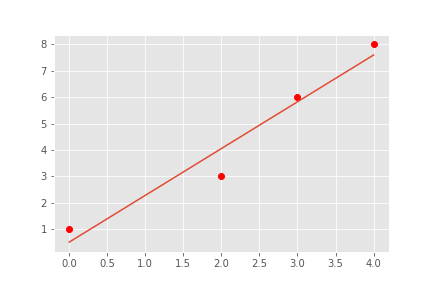
\includegraphics[]{hw1pr2c.png}
    \item 
    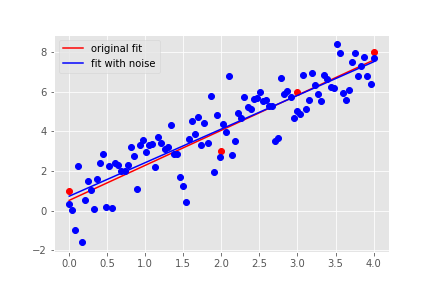
\includegraphics[]{hw1pr2d.png}
\end{enumerate}
    \vfill
\end{solution}
\newpage



\end{document}

